\documentclass{beamer}
\usepackage{tikz}
\usepackage[labelfont=bf]{caption}
\usepackage{booktabs}
\usepackage{caption}
\usepackage{siunitx}
\usepackage{amsmath}
\usepackage{pgfplots}
\usepackage{pgfplotstable}

\title{Determining the accleration due to gravity via the observation of two simple harmonic oscillators}
\author{Henry Oehlrich}

\begin{document}
\maketitle

\begin{frame}
    \frametitle{Abstract}
\end{frame}

\begin{frame}
    \frametitle{Experiment Setup}
    \begin{minipage}{0.5\textwidth}
        \begin{tikzpicture}
            \draw (-2,0) -- (2,0);
            \draw[dashed] (0,0) -- ++(0, -3);
            \draw (0,0) -- ++(-1, -2.6) node [midway, left] {\footnotesize $l$} ++(-0.2, 0) rectangle ++(0.4, -0.4) node [midway] {\footnotesize $m$};
            \draw (0,-0.5) arc [start angle=270, end angle=249, radius=5mm] ++(+0.05,-0.2) node {\footnotesize $\theta$};
        \end{tikzpicture}%
        \vspace{1cm}
        \begin{tabular}{l|l}
            \toprule
            Variable & Description \\
            \midrule
            $l$ & measured length \\
            $m$ & varied mass \\
            $\theta$ & small angle ($<$ \ang{15}) \\
        \end{tabular}
    \end{minipage}%
        \begin{tabular}{l|l}
            \toprule
            Variable & Description \\
            \midrule
            $m$ & varied mass \\
            $x$ & measured displacement \\
            $x_0$ & initial displacement \\
        \end{tabular}
        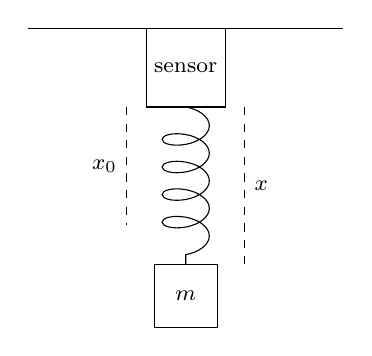
\begin{tikzpicture}
            \draw (-2,0) -- (2,0);
            \draw (-0.5,0) rectangle ++(1, -1) node [midway] {\footnotesize sensor};
            \draw[decorate, decoration={coil, segment length=3.5mm, amplitude=3mm}] (0,-1) -- ++(0, -2);
            \draw (-0.4,-3) rectangle ++(0.8, -0.8) node [midway] {\footnotesize $m$};
            \draw[dashed] (0.75,-1) -- ++(0, -2) node [midway, right] {\footnotesize $x$};
            \draw[dashed] (-0.75,-1) -- ++(0, -1.5) node [midway, left] {\footnotesize $x_0$};
        \end{tikzpicture}
    \begin{minipage}{0.5\textwidth}
    \end{minipage}
\end{frame}

\begin{frame}
    \frametitle{Materials and Methods}
\end{frame}

\begin{frame} 
    \frametitle{Results} 
\end{frame}

\begin{frame}
    \frametitle{Energy Relationship Graph}
\end{frame}

\begin{frame}
    \frametitle{Discussion}
\end{frame}

\end{document}
